\section{Theory}
\label{sec:Theory}

\subsection{Strain Sensing}
Resistance $R$ of a conducting material is governed by the equation (\ref{eq:Resistance}), where $l$ is the length, $A$ the area of the crossection and $\rho$ the electric resistivity, which inherently depends on the conducting material.

\begin{equation}
\label{eq:Resistance}
    R = \frac{l}{A}*\rho
\end{equation}

When applying transaxial strain, in most cases, a compression in transversal direction can be observed. The ration between those two forces is described by the material dependent Poisson's ratio, which in most cases ranges between 0 and 1. \cite{Gercek} In terms of conductivity-mediated strain sensing, this means, that the resulting decrease in $A = (A' -\Delta A)$ and the increase in length $l= (l' +\Delta l)$ leads to a measurable increase in resistance $R$ upon strain. In resistance-mediated strain sensing we make use of this exact dynamic.

\myworries{Add Schematic of Strain Sensing}

\subsection{Polyurethane}

Polyurethanes (PUR) are biocompatible and biostable polymers, with urethane as the characteristic group. Due to most PUR being classically synthesised using polycondensation of diisocyanates with alcohols and amines, two side groups per monomer are introduced. This leaves the option for functionalization, depending on the requirement of the application.

\begin{figure}[H]
    \centerline{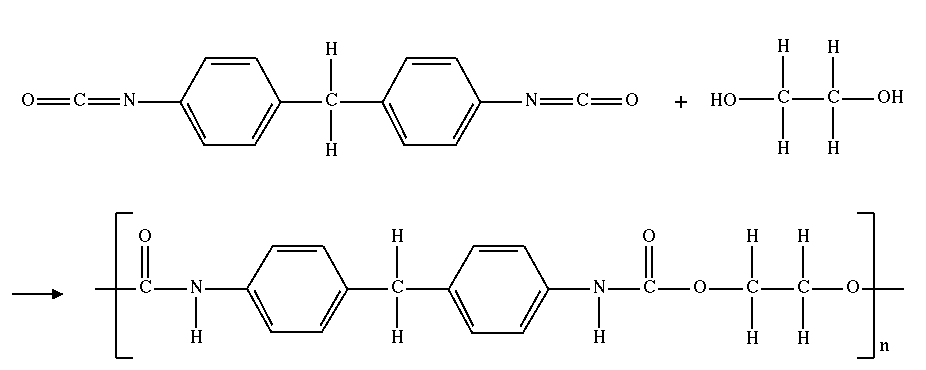
\includegraphics[scale=0.7]{./pic/Polyurethane.png}}
    \caption{Schematic of PUR-Synthesis}
    \label{fig:PURSynth}
\end{figure}

On one hand, they're moldable and have favourable tensile and fatigue properties, all of which makes them a suitable choice of material for the development of most complex biomedical devices. \cite{Pinchuk}
Until now, PUR has been extensively studied in the context of small vascular shunts and cardiac assist devices, where the thromboresistant property of the PUR fit formidable. Under most physiologic conditions, PUR are degradation resistant and can handle stresses very well \cite{Ulery}.

However, PUR, is not electrically conductive. This makes it impossible to introduce electrical functionalities without further processing of PUR, like coating or introducing charged side-groups. \myworries{Find Reference of Paper where charges have been introduced.}

\subsection{Gold Salt}
\label{subsec:GoldSalt}

\myworries{Mention that gold NP's change color depending on size. Due to plasmonics interactions in matter.}
When evaluating, which conductive material to use, noble metals seem to
host quite some promising candidates. The two main properties we wanted to
base our decision on were specific conductivity and biocompatibility.

IDEA
Focus on the specific conductivity chart suggests, that we should find 

/IDEA

As a consequence we decided on using gold, as it strikes the balance between conductivity and 
biocompatibility. \myworries{What's with other noble metals.} Also there is robust evidence, that gold stays biocompatible, even as gold nanoparticles (AuNP). \myworries{Why shouldn't it stay biocompatible as nanoparticles} This is especially important, when considering that this is the 
relevant size range for this work. \cite{Liu, Shukla}

Due to practical reasons, we had an interest in increasing the efficiency. \myworries{Rephrase/Elaborate} This is typically done by minimising the amount of substance that is wasted in non-targeted interactions. Gold in bulk is highly inert and therefore difficult to incorporate in a directed chemical approach, whereas the ionic form is a well studied agent in Redox-reactions (i.e.the method that was chosen in this work). The increase in efficiency can be achieved using a spatially selective approach, where gold salt located only in and on the fiber is reduced to become solid gold.

Gold(III) chloride trihydrate was therefore the oxidation agent of choice. \myworries{Check out other gold salts. Maybe this salt has highest potential, therefore easier to be reduced.}

\subsection{Reduction agent}
\label{subsec:RedAgent}

Redox-reactions are electrochemical reactions where electrons are exchanged between 
the participating agents. Typically the reaction is described by using two so-called 
half-reactions.The reduction half-reaction describes the process of loosing, whereas the 
oxidation counterpart describes gaining electrons, respectively. As one might expect, the 
presence of a specific half reaction to happen and the direction in which it happens (Oxidation or Reduction), depends on its inherent likelihood of happening and its relation to the likelihood of the present alternatives of half-reactions. \myworries{Rephrase.} In the Redox-regime, the likelihood is coupled to a so-called standard-reduction potential or \textsc{SRP}. Volt is the unit of the SRP and the SRP of a specific half reaction is denoted by \textit{E\textsuperscript{0}}.
The more negative the SRP of a half-reaction, the more likely the reaction 
to happen. Every half reaction is reversible and will be reversed when a half reaction with a lower \textit{E\textsuperscript{0}} is encountered. \\[0.2cm]

 \begin{center}
    \schemestart 
    \ce{[AuCl4]-} + 3$\mathrm{e^-}$  \arrow{->} \ce{Au{(s)}} + 4\ce{Cl-}, E\textsuperscript{0}\textsubscript{Gold} = +0.93 V 
    \schemestop\par 
 \end{center}
 \myworries{Maybe tweak with centerline}
 \begin{center}
     \schemestart 
    3Red \arrow{->} 3$\mathrm{Red^+}$ + 3$\mathrm{e^-}$, E\textsuperscript{0}\textsubscript{Red} $\mathrm{<}$ +0.93 V
    \schemestop\par
 \end{center}


The desired reaction to happen, is the reduction of the gold-chloride to get gold in its solid form (denoted by \ce{Au{(s)}}). Gold in bulk is electrically conductive and highly bioinert. \myworries{Consider Wojnicki }
When choosing potential candidates, we defined several qualities, which the desired reduction agent should have.

First, it should reduce gold efficiently and exclusively. On one hand, this confines the list of potentially chosen agents to those who comply with E\textsuperscript{0}\textsubscript{Red} $\mathrm{<}$ +0.93 V, according to Redox-Theory. On the other hand we want to minimise interactions between the reduction agent and PUR, due to possibly modified mechanical, chemical or biocompatible properties. This happens more often with very aggressive reduction agents, which have been shown to introduce radicals and modification of the surface properties. \myworries{Ref} Hence, we want to avoid very strong reaction agents. 

Second, we want it to be biocompatible. Since the goal of this work lies in applying knowledge in biomedical applications, the importance of biocompatibilty is given. If the reduction agents itself fulfils this requirement, then there is no need for introducing another washing-step, which could possibly introduce additional insecurities with its degree of freedom with multiple failure modes. \myworries{Ref}


Third, the reduction agent should be easily accessible and not too expensive, to facilitate access to technology and faster iterations when developing applications.

\subsection{Nucleation and Percolation}
\label{subsec:Perc}

When non-polar singular atoms of metallic species are produced in polar liquid, they want to continually aggregate to atoms of the same species, since it's energetically favourable when compared to their existence in the singular atomic state. This leads to the formation of so called embryos. \cite{Goia} But embryos still mark a non-solid-state phase, since they are subject to a continuous dissociation-aggregation process. If the system allows for an advancement through enough available free energy, eventually the embryos will grow to become nuclei. Nuclei are physically stable and don't dissociate spontaneously anymore. As the name suggest, they act as an atomic 'seed' where newly produced atoms can adhere to instead of trying to become embryos themselves. In terms of redox-reaction, this means that weaker reduction agents should lead to less but bigger nanoparticles. For stronger ones, the opposite case applies. \cite{LaMer}

To elucidate how this process is important to us, I have to introduce percolation. Percolation whose behaviour is governed by laws of Percolation Theory, describes the successful transmission of current through a random path, where each edge (air, PUR) between two nodes (gold nanoparticles) carries a probability of conducting the current. We say that something percolates if the transmission is successful from one end to the other of our sample space. The very important point here is that the exact way through which the current is conducted is not known, we only the know the probabilities. Intuitively, it becomes clear, that bigger nanoparticles have fewer but bigger overlap with other nanoparticles. This might lead to smaller resistance. However, as soon as we apply strain, those bigger nanoparticles become an uncertainty since the overall percolation depends much more on individual conduction events, leading to a broader probability-distribution, whereas in the small-but-a-lot-case the percolation distribuition is much narrower. \myworries{Reference} \myworries{taken from Wikipedia, Percolation Theory.} 

Taken those insights from nucleation and percolation together, should lead to one main insight: Namely, that stronger reduction agents, according to theoretical induction, should lead to better conductivity, when compared to weak reduction agents.

